% Chapter Template

\chapter{Implementation} % Main chapter title

\label{Chapter3} % Change X to a consecutive number; for referencing this chapter elsewhere, use \ref{ChapterX}

In this chapter we describe how we adapted the preexisting motion capture software in order to obtain the desired distorted behavior.

\section{Distortion model}


\subsection*{Linear Function}

As briefly mentioned in chapter \ref{Chapter2}, we are taking advantage of the Egocentric Coordinate formalism in order to introduce our distortion model. Formally, we modify each relative displacement vectors $\vec{v}_i$ according to a gain $\gamma$ measured in \SI{}{\decibel}. A distorted position $\vec{p}_j$ is thus obtained using equation \ref{eq:DistortionOperation}, which is modified using the one proposed by \cite{molla2017egocentric}.

\begin{equation}
\label{eq:DistortionOperation}
\vec{p}_j = \displaystyle\sum_{i=1}^{n} \hat{\lambda}\big(\vec{x}_i + f(\vec{v}_i,\gamma )\big)
\end{equation}

\noindent
And $f$ is defined as:
\begin{equation}
\label{eq:DistortionFunction}
f(\vec{v},\gamma ) = \hat{v} \cdot \norm{\vec{v}} \cdot 10^{\frac{\gamma}{10}}
\end{equation}

\noindent
Where $\vec{v}$ is a vector, $\hat{v}$ is its normalized counterpart, and $\gamma \in \mathbb{R}$. The last factor, $10^{\frac{\gamma}{10}}$, comes from the definition of a gain, in \SI{}{\decibel} \cite{book:decibel}:

\begin{align*}
    \text{gain} = \gamma &= 10 \cdot \log_{10} (\frac{P_1}{P_2})\\
    10\gamma &= \log_{10} (\text{slope})\\
    \text{slope} &= 10^{\frac{\gamma}{10}}.
\end{align*}

\noindent
A value of $\gamma = 3$ thus indicates that the virtual movement will roughly be twice the amplitude of the registered one ($1.995 \approx 2$), while a gain of $\gamma = -3$ means one will have to travel twice as much as a perceived distance in order to cover it. Figure \ref{fig:armExamples} shows two examples of distortion, and Figure \ref{fig:plotsOfGamma} gives a few instances of distortion functions with varying $\gamma $ values. This plot, as well as all the other plots of this report, were obtained using the Plotly API \cite{plotly}.

\begin{figure}
    \centering
    \begin{subfigure}[b]{0.2\textwidth}
        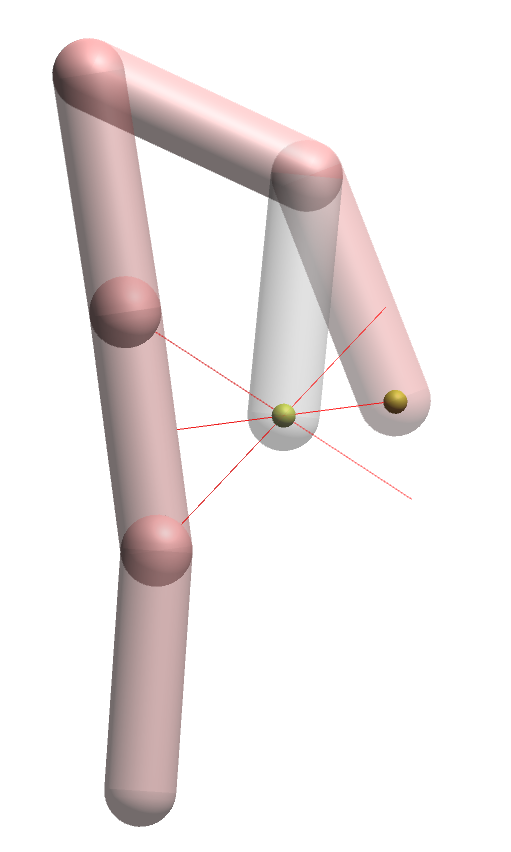
\includegraphics[width=\textwidth]{Figures/simple_distortion_3.png}
        \caption{$\gamma = 3$}
    \end{subfigure}
    ~ %add desired spacing between images, e. g. ~, \quad, \qquad, \hfill etc. 
    %(or a blank line to force the subfigure onto a new line)
    \begin{subfigure}[b]{0.2\textwidth}
        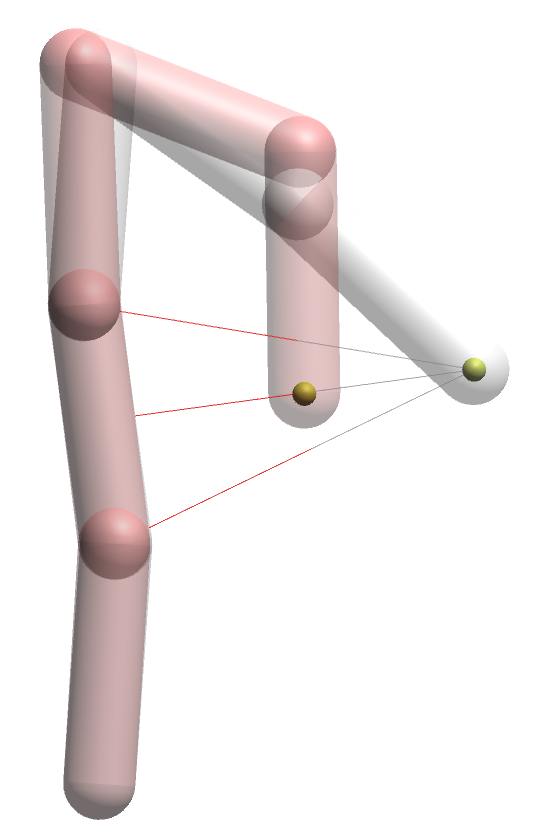
\includegraphics[width=\textwidth]{Figures/simple_distortion_-3.png}
        \caption{$\gamma = -3$}
    \end{subfigure}
    \caption{Two examples of distortion applied to a simple IK arm with multiple segments. The gray lines are the relative displacement vectors and the red ones are their distorted counterparts. Similarly, the gray arm represents the pose the real arm would take whereas the red one shows the resulting distorted pose. }\label{fig:armExamples}
\end{figure}

\begin{figure}[h]
    \center{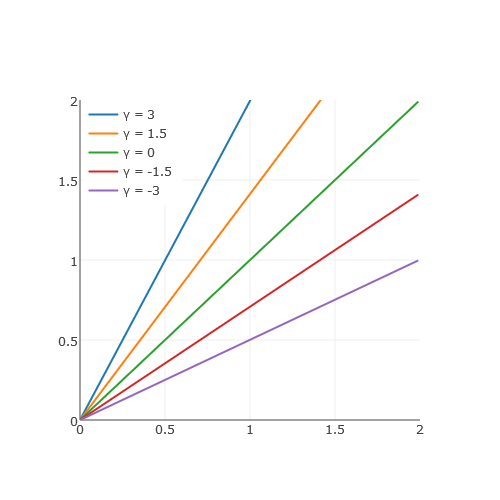
\includegraphics[width=.5676\textwidth]
    {Figures/gammaValues.png}}
    \caption{An example of a few distortion functions for various values of $\gamma $.}\label{fig:plotsOfGamma}
\end{figure}

\subsection*{Other Functions}

Before deciding to use a simple, thus easier to quantify, linear function for our experimentation process, we tried out different functions that we think are of interest for further applications. Two of these functions are described here as a reference for further investigation.
\\\\
Description and plots of the Power and Cosine functions.

\section{Egocentric Coordinates}

We added one more modification to the definition of the position proposed by \cite{molla2017egocentric} which we modified to obtain Equation \ref{eq:DistortionOperation}, and more precisely the way $\lambda $ is defined. As explained in Appendix A.4 of \cite{molla2016precise}, it is originally computed as the product of two importance factors, proximity and orthogonality respectively denoted $\lambda_p$ and $\lambda_\bot $.
\\\\
Given that the justification for the latter factor mainly relies on the semantic information it conveys, and considering that it would introduce complex behaviors in the distortion, we decided to remove it. As an example, having the hand at a given distance of the chest and changing only its orientation with respect to that body part would cause that hand's position to be affected differently by other nearby body parts and thus be altered by our distortion model.
\\\\
The former importance factor was initially defined as $\lambda_p = \frac{1}{\norm{\vec{v}}}$. In practice we find that this formula does not give enough importance to nearby body parts, and we decided to change it slightly as $\lambda_p = \frac{1}{\norm{\vec{v}}^2}$. --Mention angle solide.-- % which more closely represents the amount of surface of an object that is visible at a distance $\norm{\vec{v}}$.

\section{Reachable Sphere}

A few words on the concept of reachable sphere and how it might help at the limits of the reachable space.
